\chapter{Introduction}

% Some sort of hook, surely someone somewhere said "data is the new gold" or something

% State the argument you will make in the report

\section{Motivation}

The World Economic Forum ranked ``Failure to mitigate climate change" as the number one threat to the world in the next ten years~\cite{GlobalRisksReport}, due to the effects climate change has on extreme weather events, biodiversity, and climate-vulnerable economies. Decarbonisation is a crucial step in mitigating climate change. In New Zealand, process heat accounts for 8\% of total greenhouse emissions~\cite{DecarbonisingProcessHeat}.

Digital Twin technology shows promise in assisting decarbonisation, through efficient energy management \cite{yu2022energy}. A Digital Twin is a virtual model of a physical object or system that is connected to the real-world object or system. It can be used to monitor, control, and optimise the real-world object or system. Digital Twins are used in a variety of industries, including manufacturing, healthcare, and transportation \cite{9359733}. However, most Digital Twins in literature are designed for very specific use cases, and there is a lack of standardisation in the field.

Ahuora is a research group focused on developing smart energy systems to decarbonise factories. They have developed a Web-based simulation platform that allows users to create a digital twin of their factory.
This platform is based on steady-state simulation, which simulates a factory at a single point in time. All factory conditions are manually specified by the user.
This platform is useful for modelling changes to a factory before construction, or understanding the factory's performance under different conditions.

At the current stage of development, the Ahuora platform cannot be considered a ``Digital Twin'' because it does not take into account the factory's real-time state.
By integrating real-time sensor data into the simulation, the platform can monitor the factories' performance, and suggest tunings that will optimise resource efficiency.
The data can also be used to predict and avoid failures and downtime, a key problem where many resources are wasted.
Additionally, models created in the Ahuora Simulation Platform during the design phase could also be used during operation, minimising overhead costs.

Including real-time data in the simulation is needed to improve the usefulness of the Ahuora Platform in industry.
The system needs to meet industry requirements for security, scalability, and reliability. As such, this project
has been commissioned to develop a standardised framework to enable the integration of real-time sensor data into the Ahuora Digital Twin Platform.


\section{Objectives}

The objectives of this project are as follows:
\begin{itemize}
    % Literature review has already been conducted, so this is not necessary
    %\item Conduct a literature review on Digital Twins, Digital Twin Platforms, and Data Processing Tools.
    \item Conduct an Exploratory Analysis of techniques and tools for digital twin development, based on their applicability to the Ahuora Digital Twin Platform and the requirements of live data processing.
    \item Develop the Ahuora Digital Twin platform to a stage where support for live data processing can be added.
    \item Develop a standardised framework for integrating real-time sensor data into the Ahuora Digital Twin Platform.
    \item Develop a prototype implementation of the framework.
    \item Evaluate the prototype implementation in a case study.
    \item Identify areas for future work.
\end{itemize}
\section{Scope}

Full integration of real-time sensor data into the Ahuora Digital Twin Platform is out of scope for this project.
This project will focus on identifying techniques and tools for simulation and modelling that will be needed in a industry setting,
and developing a prototype live data processing system for Ahuora that is extensible enough to support those techniques and tools.


\section{Literature Review}

\textit{This section is a summary of the full Literature Review included in Appendix \ref{sec:litreview}}


\subsection{Data Collection in Industrial Facilities}

Real-time data is used extensively for monitoring and improving operational efficiency, particularly for schedule optimisation. It shows promise for more advanced diagnostics, fault classification, and control optimisation \cite{udugamaRoleBigData2020}. Real-time data is a crucial element of the emerging field of Digital Twins because it enables the virtual model to be aware of changing conditions in the real world.

Crucial factory tasks such as diagnostics, control, and optimisation must be peformed in real time. Software produced in this project must be reliable.
The software must be scalable enough to work in large and small industrial settings and needs to provide interoperability with existing systems that perform some of these roles already.


\subsection{Data Processing Pipeline}

In a factory, raw data is collected from SCADA systems, IoT networks, and system logs. 
This data is organised and labelled, tagging it with relevant contextual information such as timestamps and source information. Sensor data from multiple sources can then be fused together to provide more meaningful, understandable interpretations, cotributing to an increase in accuracy and fault tolerance. 
These interpretations serve as a bridge between raw data and model simulation. Simulation is used to estimate other parameters of the system that may not be able to be measured directly by sensors, enabling a comprehensive view of the entire industrial process's state. 
Finally, manually defined or data-driven algorithms can be used to respond to the process's state, to optimise schedule, control, or maintenance tasks. 
This pipeline is summarised in \Cref{fig:processing_pipeline}.

\begin{figure}[h]
    \centering
    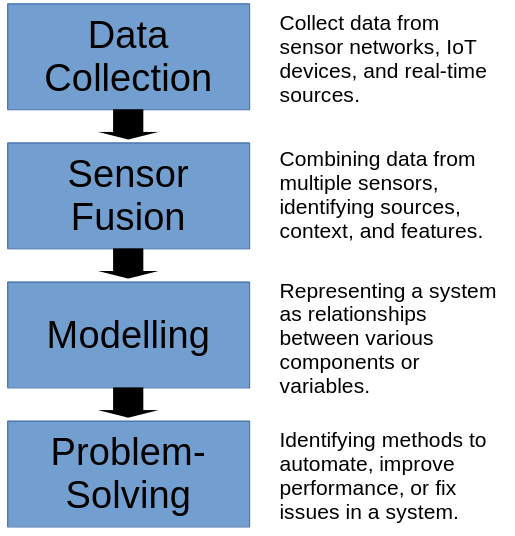
\includegraphics[width=0.4\textwidth]{LR_summary.png}
    \caption{Pipeline for processing Live Data in Digital Twin Systems, as identified in the Literature Review (Appendix \ref{sec:litreview})}
    \label{fig:processing_pipeline}
\end{figure}

This project's aim is to ingest live data from an industrial process and use a mathematical model to estimate other parameters in real-time. 
It focuses on the sensor fusion and model simulation areas of the data processing pipeline. Hence, the inputs and outputs of the project can be clearly defined.

\begin{itemize}
    \item Input: Historical \& live data from lower-level Data Collection Software, e.g SCADA systems or IoT Networks.
    \item Output: Real-time simulation results, for higher-level optimisation, control and reporting tools.
\end{itemize}

The software will be responsible for transforming measurements from sensors into a comprehensive model of the factory.

\subsection{Sensor Fusion and Hybrid Modelling}

Advanced methods for sensor fusion, such as Bayesian Analysis, Fuzzy Logic, and Theory of Evidence models, can help convert data into a more interpretable format that is appropriate for use in an analytical or mathematical model. 
Furthermore, Hybrid modelling has been shown to enable more flexible modelling that still retains the advantages of mathematical modelling. 
It is better suited to the variation and noise that is inherent in real-world sensor measurements. 
Hybrid Modelling also enables the modelling of complex dynamics that are difficult to capture via mathematical modelling alone. 
Additionally, live modelling augments models with the ability to update themselves in real time, so that the model can reflect changes in the real-world environment.


This provides a basis for developing the core features required in the Ahuora Platform. The platform needs to incorporate existing or novel sensor fusion technologies to prepare data for modelling. 
The Ahuora Platform is built on the IDAES process simulation engine. Further research is required to understand how IDAES supports hybrid modelling, and how to make hybrid modelling feasible in a real-time context.
The optimal technologies and methods to use for hybrid modelling in real-time is also uncertain, so further research is likewise required to investigate this. 
This research needs to be conducted within the context of the needs and requirements of the Ahuora Platform, to ensure that the approach also supports the broader goals of the Ahuora project.

